\documentclass{article}
\usepackage{graphicx}
\usepackage[margin=1.5cm]{geometry}
\usepackage{amsmath}
\usepackage{hyperref}

\begin{document}
\twocolumn

\title{Combining Theoretical, Simulated, and Experimental Physics}
\author{Prof. Jordan C. Hanson}

\maketitle

\section{Theoretical Prediction: Pendulum}

\begin{enumerate}
\item A \textit{pendulum} is a device we can use to measure the effect of gravity, and to study forces in general.
\item Let the horizontal displacement of a pendulum be $x(t)$, with a maximum displacement $x_0$, in units of cm.  Further, let $\omega$ and $\phi$ have units of radians/s and radians, respectively. The motion of a pendulum (Fig. \ref{fig:pendulum}) theoretically follows Eq. \ref{eq:1}:
\begin{equation}
x(t) = x_0\cos(\omega t + \phi) \label{eq:1}
\end{equation} 
\begin{figure}[ht]
\centering
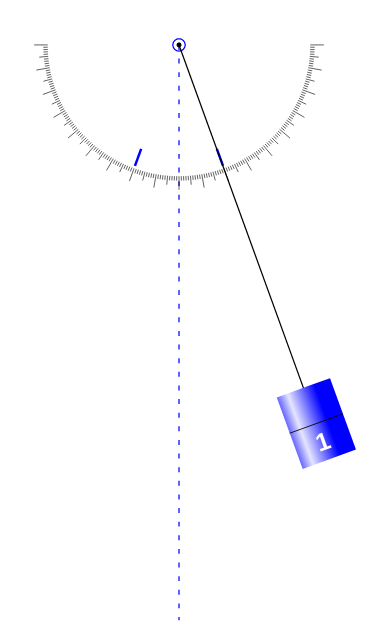
\includegraphics[width=0.15\textwidth]{pendulum.png}
\caption{\label{fig:pendulum} A pendulum is a mass $m$ that swings on a chord of length $L$ with angular frequency $\omega = \sqrt{g/L}$, where $g$ is the acceleration due to gravity.}
\end{figure}
\item Suppose $\phi = 0$, $\omega = 2\pi/3$ rad/s, and $x_0 = 4$ cm.  (a) What is the displacement at $t=3/2$ seconds? (b) When is $x(t) = 0$? (c) What is the maximum positive displacement? \\ \vspace{2cm}
\item The \textit{period} of the pendulum is the time duration required to observe the pendulum return to the same state.  Point your browser to the following link: \url{https://phet.colorado.edu/en/simulations/pendulum-lab}.  Using the Intro tab of this PhET, and a spreadsheet program, create a table of the \textit{period} of the pendulum in seconds, versus the \textit{length} of the pendulum in centimeters.  Sketch a graph of the data below. \\ \vspace{2cm}
\end{enumerate}

\section{Lab Measurement}

\begin{enumerate}
\item Using the pendulum at your lab table, \textit{collect the same data points as your simulation.}
\item Graph the simulated and observed period ($T$) on the same graph.  Add the following theoretical expectation, using $g = 9.81$ m s$^{-2}$, and lettiong $L$ be the pendulum length in \textit{meters}.
\begin{equation}
T = 2\pi \sqrt{L/g}
\end{equation}
\item Discuss how well your lab data, simulation data, and theoretical expectation match.
\end{enumerate}

\end{document}
